\chapter{Related Work}


\section{Graph Theory Basics}

In this section some graph theory related notation is defined which is used during this thesis.
It is for the most part based on~\cite{Thulasiraman1992} and on~\cite{Diestel2012}.
A graph is a mathematical construct that can be used to model and explore the relationship between objects.
More formally, a graph is a ordered pair of finite sets \(G = (V, E)\), whereas \(V\) denotes the set of \emph{vertices} (i.e., the objects) and \(E \subseteq [V]^{2} \) the set of \emph{edges} (i.e., the relationships between the objects).
It is common to write \(V(G)\) and \(E(G)\) to refer to the set of vertices, respectively the set of edges, that are associated with a graph \(G\).
An edge \(\{v_1, v_2\} \in E(G)\) is an unordered pair of two vertices.
This means that there is no distinction between the two edges \(\{v_1, v_2 \}\) and \(\{v_2, v_1\}\).
A graph with this property is called a \emph{undirected} graph.
However, it is also possible to define edges as ordered pairs, so that each edge does have a start- and endpoint.
Such a graph is called a \emph{directed} graph.
An edge of the form \(\{v_i, v_i\} \in E(G)\) is called a \emph{self-loop} of the vertex \(v_i\).
Furthermore, it is possible that two distinct vertices are joined by multiple edges.
Such edges are referred to as \emph{parallel} edges.
A graph that has no parallel edges and no self-loops is called a \emph{simple} graph.
Figure~\ref{fig:example_graphs} depicts a example for a simple graph and for a graph with multiple edges and a self-loop vertex.
All further mentions and definitions for graphs are referring to undirected simple graphs unless stated otherwise.

\begin{figure}[h]
   \centering
   \begin{subfigure}[t]{0.45\textwidth}
     \centering
     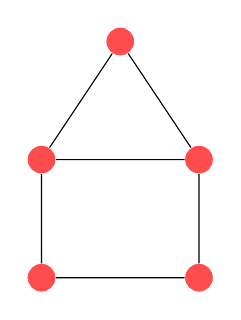
\begin{tikzpicture}[node/.style={circle,fill=red!70,minimum size=1em,inner sep=3pt]}]
       \node[node] (1) at (0, 0) {};
       \node[node] (2) at (-1, -1.5)  {};
       \node[node] (3) at (1, -1.5) {};
       \node[node] (4) at (-1, -3) {};
       \node[node] (5) at (1, -3) {};

       \draw (1) -- (3);
       \draw (1) -- (2) -- (4) -- (5) -- (3) -- (2);
     \end{tikzpicture}
     \caption{A undirected simple graph.}
   \end{subfigure}
   ~
   \begin{subfigure}[t]{0.45\textwidth}
     \centering
     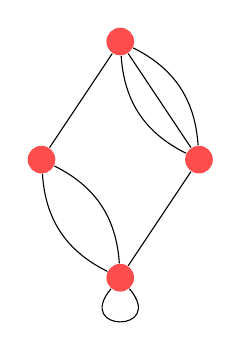
\begin{tikzpicture}[every loop/.style={}, node/.style={circle,fill=red!70,minimum size=1em,inner sep=3pt]}]
       \node[node] (1) at (0, 0) {};
       \node[node] (2) at (-1, -1.5)  {};
       \node[node] (3) at (1, -1.5) {};
       \node[node] (4) at (0, -3) {};

       \draw (1) -- (2);
       \draw (1) -- (3) -- (4);
       \path (2) edge [bend left] (4);
       \path (2) edge [bend right] (4);
       \path (3) edge [bend left] (1);
       \path (3) edge [bend right] (1);
       \draw (4) edge [in=-50,out=-130,loop] (4);
     \end{tikzpicture}
     \caption{A undirected graph with a self-loop and parallel edges.}
   \end{subfigure}

   \caption[Examples for graphs]{Graphical representation of two graphs with different properties.
   The vertices are represented by red dots and the edges are the line segments between them.}
\label{fig:example_graphs}
\end{figure}


The \emph{order} of a graph is its number of vertices (i.e., the cardinality of the vertex set) and is denoted as \(n = |V(G)|\).
The neighborhood of a vertex \(v_i\) is defined as \(N(v_i) = \{v_j \in V(G) : \{v_i, v_j \} \in E(G)\}\).
It is the set of vertices that are \emph{adjacent} to the vertex \(v_i\).
The cardinality of this set is called the \emph{degree} of the vertex and is denoted as \(d(v_i) = |N(v_i)|\).
A vertex without any neighbors (i.e., with a degree of zero) is called \emph{isolated}.
It is also often very useful to measure degree properties for the graph.
For example, the \emph{minimum degree} \(\delta(G) = \min\{d(v_i) : v_i \in V(G)\}\), the \emph{maximal degree} \(\Delta(G) = \max\{d(v_i) : v_i \in V(G)\}\), and the \emph{average degree} \(d(G) = \frac{1}{n} \sum_{v_i \in V(G)} d(v_i)\).
Another way to calculate the average degree is \(d(G) = \frac{2|E|}{n}\), due to the fact that each edge is counted twice during the summation of the vertex degrees.
These global measures can be used to get an insight in the basic structure of the graph.
Another global property related to the degree is the \emph{degree distribution} \(p\)~\cite{Barabasi2016} of a graph.
It yields the probability that that a randomly selected vertex has a degree of \(k\).
Since it is a probability distribution \(\sum_{k=0}^\infty p(k) = 1\) must hold.
The degree distribution for a given graph can be calculated by using \(p(k) = \frac{|\{v \in V(G) \,:\, d(v) = k\}|}{n}\) (i.e., calculating the normalized histogram).

A \emph{path} on a graph can be defined as a finite sequence of vertices \(v_1,v_2,\dots,v_k\), such that between any consecutive pair of vertices exist a edge in the graph.
Furthermore, all edges between the vertices and the vertices itself must be distinct.
The first and the last vertices in the sequence are called the \emph{end vertices} or \emph{terminal vertices} of the path.
The \emph{path length} is the number of edges on the path.
Two vertices are \emph{connected} if it is possible to find a path with these two vertices as end points.
A vertex is, by definition, connected to itself.
If there exists a path between all pairs of vertices, then the graph is called connected.
It is possible to partition the vertex and edge set of a not connected graph in such a way that there are no edges between vertices in different partitions.
These partitions are called the \emph{components} of the graph.

The \emph{clustering coefficient}~\cite{Watts1998} of a vertex is a measure for the cliquishness of its neighborhood.
A \emph{clique} in a graph is a subset of vertices, such that there exists an edge between every pair of vertices in this set.
The clustering coefficient \(C(v_i)\) is defined as the fraction of possible edges between the neighbors of the vertex \(v_i\).
There are at most \(\binom{d(v_i)}{2} = \frac{d(v_i)(d(v_i) - 1)}{2}\) possible edges between vertices in the neighborhood.
Therefore, the clustering coefficient can be calculated using equation~\ref{eq:clustering-coefficent}.

\begin{equation}
 C(v_i) =  \frac{2 \, |\{\{v_j, v_k\} \in E(G) : v_j \in N(v_i) \wedge v_k \in N(v_i)\}| }{d(v_i)(d(v_i) - 1)}
 \label{eq:clustering-coefficent}
\end{equation}

This is, of course, a local property of one vertex.
However, it is also often useful to consider the average clustering coefficient \(C = \frac{1}{n} \sum_{v(i) \in V(G)} C(v_i)\) of the graph.
Figure~\ref{fig:clustering-coefficent-examples} shows some examples for neighborhoods with different clustering coefficients.


\begin{figure}[h]
   \centering
   \begin{subfigure}[t]{0.31\textwidth}
     \centering
     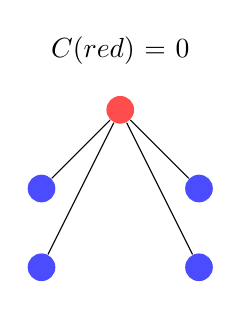
\begin{tikzpicture}[node/.style={circle,fill=red!70,minimum size=1em,inner sep=3pt]}, neighbor/.style={circle,fill=blue!70,minimum size=1em,inner sep=3pt]}]
       \node[text width=6em, align=center] at (0, 0.75)  {\(C(red) = 0\)};
       \node[node] (1) at (0, 0) {};
       \node[neighbor] (2) at (-1, -1)  {};
       \node[neighbor] (3) at (1, -1) {};
       \node[neighbor] (4) at (-1, -2)  {};
       \node[neighbor] (5) at (1, -2) {};

       \foreach \p in {2,3,4,5}{\draw (\p) -- (1); }
     \end{tikzpicture}
     \caption{In this example none of the four neighbors shares a edge with any other neighbor of the red vertex.
     Therefore, the clustering coefficient of the red vertex is \(\frac{0}{6} = 0\).}
   \end{subfigure}
   ~
   \begin{subfigure}[t]{0.31\textwidth}
     \centering
     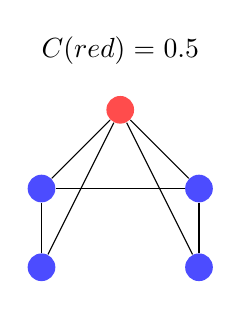
\begin{tikzpicture}[node/.style={circle,fill=red!70,minimum size=1em,inner sep=3pt]}, neighbor/.style={circle,fill=blue!70,minimum size=1em,inner sep=3pt]}]
       \node[text width=6em, align=center] at (0, 0.75)  {\(C(red) = 0.5\)};
       \node[node] (1) at (0, 0) {};
       \node[neighbor] (2) at (-1, -1)  {};
       \node[neighbor] (3) at (1, -1) {};
       \node[neighbor] (4) at (-1, -2)  {};
       \node[neighbor] (5) at (1, -2) {};

       \foreach \p in {2,3,4,5}{\draw (\p) -- (1); }
       \draw (2) -- (4);
       \draw (3) -- (5);
       \draw (3) -- (2);
     \end{tikzpicture}
     \caption{Here are half of the possible edges between the neighbors are present.
     The clustering coefficient of the red vertex is \(\frac{3}{6} = \frac{1}{2}\).}
   \end{subfigure}
   ~
   \begin{subfigure}[t]{0.31\textwidth}
     \centering
     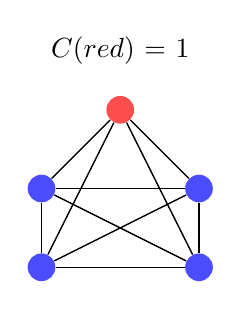
\begin{tikzpicture}[node/.style={circle,fill=red!70,minimum size=1em,inner sep=3pt]}, neighbor/.style={circle,fill=blue!70,minimum size=1em,inner sep=3pt]}]
       \node[text width=6em, align=center] at (0, 0.75)  {\(C(red) = 1\)};
       \node[node] (1) at (0, 0) {};
       \node[neighbor] (2) at (-1, -1)  {};
       \node[neighbor] (3) at (1, -1) {};
       \node[neighbor] (4) at (-1, -2)  {};
       \node[neighbor] (5) at (1, -2) {};

       \foreach \p in {1,2,3,4,5}{ \foreach \q in {1,2,3,4,5}{\draw (\p) -- (\q); }}
     \end{tikzpicture}
     \caption{The neighbors of the red vertex form a clique.
     Hence, the clustering coefficient of the red vertex is \(\frac{6}{6} = 1\).}
   \end{subfigure}

   \caption[Clustering coefficent examples]{Examples for the clustering coefficient of a vertex with a small neighborhood.
   The blue vertices are the neighbors of the red vertex.
   The possible number of edges between the four neighbors is \(\binom{4}{2} = 6\).}
\label{fig:clustering-coefficent-examples}
\end{figure}


%% ========================================================================
%% ========================================================================


\section{Social Networks}

In the real-world it is common to use graphs to model the complex systems that are arising.
For example, the web can be represented as a graph, where the vertices correspond to websites and the edges are the hyperlinks between them.
Another use case are large infrastructure networks, such as power grids.
In a graph that represents such a power grid network vertices represent things like power stations or transformers and edges the power lines between them.
However, when modeling these large networks it common to use a slightly different terminology~\cite{Barabasi2016}.
Vertices are often called \emph{nodes} and edges are called \emph{links} in the context of networks.

Social networks~\cite{Newman2010} are another type of network that can benefit from the usage of graph theory methods.
The study of these networks is considered to be a part of the field of sociology and researchers may also use slightly different terminology for the vertices and edges in their work.
Nodes (or vertices) often represent people in social networks and are also sometimes referred to as \emph{actors}.
However, it is also possible that nodes depict other entities, such as a departments, companies, or countries (i.e., larger groups of people).
The links (or edges) between these entities can mean, depending of the context, different things as well and are sometimes also referred to as \emph{ties}.
For example, links between persons can show social relationships (e.g., friendships), collaborations in projects (e.g., co-authorship of a scientific papers), or other social interactions.
Links between companies could represent trading relationships or the like.
Often social networks are only mentioned in relation to large online communities, such as Facebook or Twitter, but there is no necessity that a social network must exist in an online form.
The network of acquaintances or friends in a school is also considered as a social network.
Figure~\ref{fig:karate-club-network} shows a famous example of a small real-world social network.

\myfig{karate_club_network}
      {width=0.6\textwidth,height=0.6\textheight}
      {Zachary's karate club network~\cite{Zachary1977} is a social network that shows the relationship between 34 members of a university-based karate club in the US in the early 1970's.
      There exists an edge between two members if there were social interactions outside of the normal club activities (i.e., two members are considered as friends).
      The graph shows a separation into two groups (red and blue nodes) due to a dispute in the club.}
      {Zachary's karate club network}
      {fig:karate-club-network}

Two fundamental terms in social network analysis are \emph{dyads} and \emph{triads}~\cite{Wasserman1994}.
These two concepts describe the relationship between multiple actors.
A \emph{dyad} denotes the linkage between a pair of actors.
It is a very common research topic to understand the pairwise relationships in social networks.
A \emph{triad} on the other hand describes triples of actors and the ties between them.
This concept is especially important for the question of transitivity of certain relationships.
A example for this would be the question \enquote{is the friend of my friend also my friend?}.

A property of many real-world social networks is a \emph{community structure}~\cite{Girvan2002}.
Communities are groups of actors that are more connected to actors in the same group, than to actors in a different one.
This basically means that there exists subsets of densely linked nodes in the network with very few links to other subsets.
The network shown in figure~\ref{fig:karate-club-network} has two known communities characterized by different node colors.
The detection of community structures in networks is a very import research topic, since the identified communities may correspond to actual social groupings.
For example, the detected communities in a social network that models the friendship between students may represent the real corresponding social groups (i.e., the circles of friends).
There is a variety of different methods and approaches to perform this task.
Examples are approaches based on hierarchical clustering, or edge betweenness (i.e., the number of shortest paths going through an edge).

Another attribute that many social networks share is that they are \emph{scale-free networks}~\cite{Barabasi2016}.
Formally, a network is a scale-free network if its degree distribution is a \emph{power-law distribution} (i.e., \(p(k) \sim k^{-\gamma}\), where \(\gamma\) is the parameter of the distribution that denotes the degree exponent).
The value for \(\gamma\) for most real-world (social) networks is in the range between 2 and 3.
A consequence of the power-law distribution is that the distribution of the degrees is right-skewed with a long tail.
This means that there is a large number of nodes in the network that have only a few links (i.e., a small degree) but there is also the chance that there exists a few nodes with a very high degree.
Such nodes are usually called \emph{hubs} and may correspond in the context of social networks to very influential actors that can play an important role in the network.


%% ========================================================================
%% ========================================================================


\section{Time-varying Networks}

This section contains an overview on the concept of time-varying networks~\cite{Holme2012, Holme2015}.
Since this type of network is used in many different scientific fields it also has a variety of names.
For example, temporal networks, dynamic networks, evolving graphs, or the name that is mainly used in this thesis, time-varying networks.
As already mentioned in the section about social networks, the structure, or topology, of networks can be used to understand dynamic processes and their behavior.
However, there are a lot of dynamical processes that are modeled using networks, in which the links are not active all the time.
One example would be a communication network, such as the network of phone calls between users.
Another example would social or collaboration network, where actors do not interact constantly but in irregular intervals.
These link activation at certain times can, however, be very important to explain the dynamic process and are simply lost when approximated by a static graph.
So the idea of time-varying networks is to introduce another dimension (i.e., time) to the network and move the information of when something happens from the dynamic process to the network itself.

The usage of static networks in models for dynamic processes often results in a loss of information, that can be regained using time-varying networks.
However, these temporal networks also introduce more complexity to the model and one have to weight the gain of information versus the extra effort.
Especially in the case that the knowledge of how often something between two actors in the network happens is more important than when exactly something happens is a use case for weighted networks~\cite{Newman2010}.
This type of network introduces a mapping between the set of edges and values that represent the strength of the link.
See \autoref{fig:weighted-network-example} for an illustration of a simple weighted network.
As a general rule, a time-varying network is applicable when the structure (i.e., the topology) of the system and the temporal process are connected to each other.
This means that the time scale on which the network itself evolves should be similar to the time scale of the dynamic process that takes place on it.
For example, a time-varying network is not a suitable model for the internet, since the the infrastructure (i.e., the topology) changes very slowly in comparison to the transmission of the packages that are routed through the network (i.e., the dynamic process).

The underlying concept of time-varying networks is called \emph{contacts} and can be seen as interactions between two nodes at a certain time.
The duration of the interaction is negligible and thus assumed to be instantaneous.
Contacts can be interpreted as an extension of links in the static network.
The unordered pair \(\{v_{i}, v_{j}\}\) becomes a ordered triple \((v_{i}, v_{j}, t)\).
The order is in this case important, since the third object in the triple must refer to the interaction time \(t\) between the nodes \(v_{i}\) and \(v_{j}\).
This also means that a time-varying network cannot be represented by a graph.
Nevertheless, there are many different possibilities to represent a temporal network.
The simplest way to to this is by using contact sequences.
A contact sequence is simple a list that contains the contact triples.
This is a very raw form data (i.e., basically a spreadsheet with three columns) and is therefore very easy to parse and to use in algorithms, but is not very well suited for the analysis of the underlying dynamic process by humans due to the lack of illustrations.
Another way to represent time-varying networks are graph sequences.
The idea here is to generate a static graph that contains all contacts between nodes for a given time step.
This method has the advantage that all tools that work for static graphs can be applied to each of the graphs in the sequence.
The problem with this representation is, that the time resolution should be rather low to avoid the creation of graphs with no, or only a few, edges for most time steps.
\autoref{fig:graph-sequence-example} depicts an example of a graph sequence for a time-varying network with four nodes.
There are also more visual-focused representation methods.
One example would be assigning a time series of time stamp of the contacts between two nodes to the corresponding link in the static network (see \autoref{fig:time-stamp-edges-example} for an example).
This allows the usage of the variety of graph layout algorithms to visualize the network, but does not work very well for large networks due to the lack of space for the time stamps on the links and the large numbers of nodes.
Another idea is to visualize the time-varying network using a timeline of contacts.
The interactions between nodes (i.e., the tuple of nodes that are interacting with each other) are placed on one axis and the time is placed on the other one.
A marker is placed for each pair that interacts at a certain time.
This allows the visual detection of interaction patterns.
However, similar to the last representation methods, this one also only reasonable for small networks.
\autoref{fig:timeline-example} shows an example for this type of representation.

\begin{figure}
   \centering
   \begin{subfigure}[t]{0.39\textwidth}
     \centering
     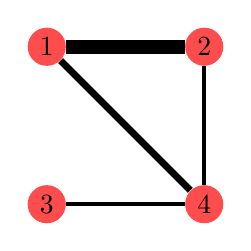
\begin{tikzpicture}[node/.style={circle,fill=red!70,minimum size=1em,inner sep=2pt]}]

       \node[node] (1) at (0, 2) {1};
       \node[node] (2) at (2, 2) {2};
       \node[node] (3) at (0, 0) {3};
       \node[node] (4) at (2, 0) {4};

       \draw[line width=5.00pt] (1) -- (2);
       \draw[line width=2.50pt] (1) -- (4);
       \draw[line width=1.25pt] (2) -- (4);
       \draw[line width=1.25pt] (3) -- (4);
     \end{tikzpicture}

   \caption{Static approximation of the contact sequence as a weighted network.
   The width of the lines between the nodes represent the strength (i.e., the weight) of the edges.
   The thicker the line the higher the weight.}
   \label{fig:weighted-network-example}
   \end{subfigure}
   ~
   \begin{subfigure}[t]{0.58\textwidth}
     \centering
     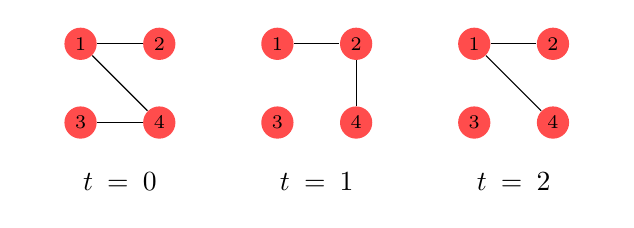
\begin{tikzpicture}[node/.style={circle,fill=red!70,minimum size=1em,inner sep=2pt]}]

       \foreach \t in {0, 1, 2} {
           \node[text width=6em, align=center] at (0.5+\t*2.5, -0.75)  {\(t=\t\)};
           \node[node] (1_\t) at (0+\t*2.5, 1) {\scriptsize 1};
           \node[node] (2_\t) at (1+\t*2.5, 1) {\scriptsize 2};
           \node[node] (3_\t) at (0+\t*2.5, 0) {\scriptsize 3};
           \node[node] (4_\t) at (1+\t*2.5, 0) {\scriptsize 4};
       }

       \draw (1_0) -- (2_0);
       \draw (1_0) -- (4_0);
       \draw (3_0) -- (4_0);
       \draw (2_1) -- (4_1);
       \draw (1_1) -- (2_1);
       \draw (1_2) -- (2_2);
       \draw (1_2) -- (4_2);
     \end{tikzpicture}

   \caption{Visualization of the graph sequence representation of the three time steps of a time-varying network.
   There exists an edge in a graph at time \(t\) if there was a contact between the two nodes at this time step.}
   \label{fig:graph-sequence-example}
   \end{subfigure}

   \begin{subfigure}[t]{0.39\textwidth}
     \centering
     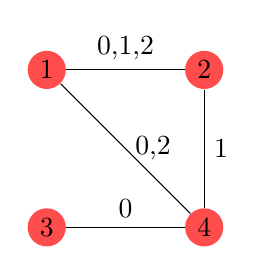
\begin{tikzpicture}[node/.style={circle,fill=red!70,minimum size=1em,inner sep=2pt]}]

       \node[node] (1) at (0, 2) {1};
       \node[node] (2) at (2, 2) {2};
       \node[node] (3) at (0, 0) {3};
       \node[node] (4) at (2, 0) {4};

       \draw (1) -- (2) node[midway, above] {0,1,2};
       \draw (1) -- (4) node[midway, right] {0,2};
       \draw (2) -- (4) node[midway, right] {1};
       \draw (3) -- (4) node[midway, above] {0};
     \end{tikzpicture}

   \caption{A graph that contains an edge between two nodes if there was at least one contact between them.
   Furthermore, the edges are annotated with a time series of time steps that indicate when the interactions took place.}
   \label{fig:time-stamp-edges-example}
   \end{subfigure}
   ~
   \begin{subfigure}[t]{0.58\textwidth}
     \centering
     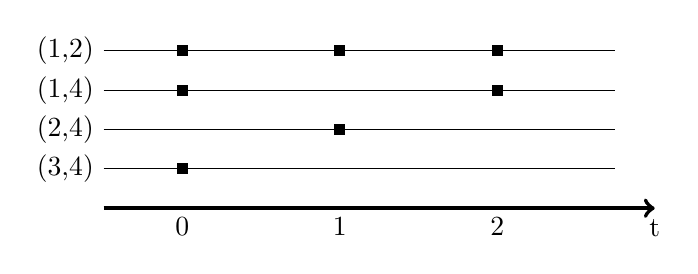
\begin{tikzpicture}[contact/.style={rectangle,fill=black,inner sep=0pt,minimum size=4pt]}]

       \draw (0, 2) node[left] {(1,2)} to (6.5, 2);
       \draw (0, 1.5) node[left] {(1,4)} to (6.5, 1.5);
       \draw (0, 1) node[left] {(2,4)} to (6.5, 1);
       \draw (0, 0.5) node[left] {(3,4)} to (6.5, 0.5);

       \draw[->, line width=1.5pt] (0, 0) to (7, 0) node[below] {t};
       \node[below] at (1, 0) {0};
       \node[below] at (3, 0) {1};
       \node[below] at (5, 0) {2};

       \node[contact] at (1, 2) {};
       \node[contact] at (1, 1.5) {};
       \node[contact] at (1, 0.5) {};
       \node[contact] at (3, 2) {};
       \node[contact] at (3, 1) {};
       \node[contact] at (5, 2) {};
       \node[contact] at (5, 1.5) {};
     \end{tikzpicture}

   \caption{Visualization of the contact sequence as a timeline of contacts.
   The vertical axis shows the interactions that happened between the nodes in the network and the horizontal axis shows the three time steps.
   There is a marker, depicted as a black rectangle, if there was a contact between the pair at a given time \(t\).}
   \label{fig:timeline-example}
   \end{subfigure}

   \caption[Graphical representations of time-varying networks]{Figures \subref{fig:graph-sequence-example}--\subref{fig:timeline-example} show different visualizations for the contact sequence \((1, 2, 0), (1, 4, 0), (3, 4, 0), (1, 2, 1), (2, 4, 1), (1, 2, 2), (1, 4, 2)\).
   Figure \subref{fig:weighted-network-example} shows a static network of the same contact sequence where the number of contacts between two nodes is reflected by the edge weights.}
\end{figure}

\todo{fix different sizes for nodes in subfigures (a) and (c)}

It is also noteworthy that most of the introduced measures for networks do not apply for temporal networks or must be redefined, respectively extended.
For example, the concept of degree distributions does not exists in this context.
But there are new measures like the \emph{inter-contact time distributions}, which describe the frequency of the time between contacts between either a specific pair of nodes or any two nodes.
Paths also cannot be used in temporal networks and are replaced by measures like \emph{latency} (i.e., how long since the last contact between two nodes) or \emph{temporal distance} (i.e., how long does it take to get from one node to another while taking the contacts into account).
There is also the idea, and many approaches, to extend community detection mechanisms for the usage in time-varying networks by running community detection algorithms for a static approximation of the network at time \(t\) and then including community information from previous time steps.


%% ========================================================================
%% ========================================================================


\section{Network Models}

This section contains descriptions of different network models.
These models can be used to build graphs that fulfill different properties.
They are often a useful tool to model some type of real-world network (e.g., a social network) to gain a deeper understanding on the processes that create these networks.

\subsection{The Erdős-Rényi Model}

The Erdős–Rényi (ER) model~\cite{Erdos1959, Newman2010} was in its first form described by the two famous mathematicians Paul Erdős and Alfréd Rényi in 1959.
The model generates a random graph with \(n\) nodes and \(m\) links.
It chooses one of the \(\binom{\binom{n}{2}}{m}\) possible graphs of this size with equal probability at random.
The idea is that large, complex networks often seem random and can be examined using random graphs and statistical methods~\cite{Barabasi2002}.
Therefore,this is a very simple, yet powerful, model to explore some effects that take place in real-world systems.
It is also often called \(G(n, m)\).
There is another model that is very similar to the \(G(n, m)\) model, called the \(G(n, p)\) model.
Here is the number of links not fixed beforehand, but determined by \(p\), the probability of the presence of a link between any pair of nodes in the network.
Hence, the edges of a random network are determined by flipping a biased coin for each of the \(\binom{n}{2}\) possible edges.

The probability for an arbitrary network with exactly \(m\) links under this model is \(p^{m} (1-p)^{\binom{n}{2} - m}\).
Therefore, the probability that the model will generate a network with \(m\) links is \(\prob{m} = \binom{\binom{n}{2}}{m} p^{m} (1-p)^{\binom{n}{2} - m}\) (i.e., the probability of such network times the number of possible networks).
This corresponds to  a binomial distribution \(B(\binom{n}{2}, p)\).
One simple consequence of that is that the expected value for the number of links \(\expval{m} = \sum_{m=0}^{\binom{n}{2}} m \prob{m} = \binom{n}{2} p\).
The expected value for the average degree of a network generated with this model is deduced in equation~\ref{eq:avg-degree-erdos-model}.
This value is also often called \(c\).
The probability that an arbitrary node has a degree of exactly \(k\) is given by \(p(k) = \binom{n-1}{k} p^{k} (1-p)^{n-1-k}\) (i.e., \(k\) of its possible \(n-1\) links must exist and there are \(\binom{n-1}{k}\) possible combinations for the \(k\) links).
Therefore, the degree distribution of this model is a binomial distribution as well.
However, it is also possible to approximate the degree distribution with an Poisson distribution \(p(k) = e^{-c} \frac{c^{k}}{k!}\) for large values of \(n\).

\begin{equation}
  c = \expval{d(G)} = \sum_{m=0}^{\binom{n}{2}} \frac{2m}{n} \prob{m} = \frac{2}{n} \sum_{m=0}^{\binom{n}{2}} m \prob{m} = \frac{2}{n} \binom{n}{2} p = (n-1) p
  \label{eq:avg-degree-erdos-model}
\end{equation}

A nice property of the Erdős–Rényi model is that it can be used to study the formation of giant components in networks.
A \emph{giant component} is a component that contains a large fraction of the nodes.
It is interesting that even such a simple model can be used to study a phenomenon that is part of many real-world networks.
However, there are also quite a few problems with this model.
The degrees in real-world networks are usually not binomial, respectively Poisson, distributed.
The formation of hubs in networks usually requires a power-law degree distribution.
Other examples for a shortcomings of the model is the inability to generate community structures and inadequate average path lengths.


\subsection{The Barabási-Albert model}

One model that addresses the problem of missing power-law degree distributions is the Barabási-Albert (BA) model~\cite{Barabasi2002}.
The model is named after its creators Réka Albert and Albert-László Barabási.
It tries to emulate the dynamic process that is responsible for the creation of scale-free degree distributions and yields a the generated network as result.
One of the main differences to the ER model is that the size of the network is not fixed.
The model starts with an small number of nodes and adds new nodes to the network over time (i.e., the network grows).
A newly added node then forms links with already existing nodes.
Which other nodes are chosen depends on how important the other nodes are.
The more important a node is, the more likely it is that the new nodes forms a connection with it.
This process is called \emph{preferential attachment}.
It can, for example, be used to describe the behavior of new users in social networks (i.e., new users tend to form ties with already established users) or that new websites on the web link to already popular ones because they are easier to find \todo{find better examples with references to papers?}.
More formally, the model starts with a small number \(m_{0}\) of nodes and the following two steps are repeated in every time step:

% examples at:http://barabasi.com/networksciencebook/chapter/5#origins

\begin{enumerate}
    \item add a new node to the network
    \item choose \(m \leq m_{0}\) already existing nodes at random proportional to their degree and form a link with them
\end{enumerate}

This means that in this model the degree of a node is a measure of its popularity  and a existing node \(v_{i}\) will be selected with a probability \(\Pi(v_{i})=\frac{d(v_{i})}{\sum_{j} d(v_{j})}\) to form a link.
The process yields after \(t\) time steps a network that consists of \(m_{0} + t\) nodes and \(mt\) links.

It can be shown, using different methods (e.g., continuum theory, master equations, and numerically), that the node degrees follow a power-law distribution with an degree exponent of \(\gamma = 3\).
Furthermore, asymptotically does \(\gamma\) not depend on \(m\), the number of links that are generated in each iteration.
The degree distribution is also (asymptotically) independent on the time, and therefore on the size of the network.
This is also a property of the model and reflects the fact that there exists real-world networks with a power-law degree distribution with different sizes.
However, like the ER model, the BA model has its shortcomings as well.
For example, the average path length of generated networks does not comply with real-world networks.
However, they are more realistic than the path lengths generated by the ER model.
Another property that cannot be reproduced by this model are the community structures that many real-world, and especially social, networks have~\cite{Reid2011}.

Another interesting question regarding the Barabási-Albert model is if both used mechanisms, the network growth and the preferential attachment, are necessary to produce a scale-free network.
The result of numerical simulations and formal tests of the model with either of the two mechanisms missing is that both are required.
Missing preferential attachment results in exponentially distributed node degrees and the missing network growth leads to a power-law degree distribution in the beginning, but it changes to a normal distribution over time.
This indicates that in fact both mechanisms are required to yield a network with the scale-free property.


%% ========================================================================
%% ========================================================================


\section{User Activity Models}
